\section{Methodological and Theoretical Framework}
\subsection{Cognitive Sovereignty and Thermodynamics: Definition and Implications}

From the thermodynamic analysis and archaeological evidence emerges a pattern of architectural transformation: the systematic collapse of sphere-like cognitive structures into vector-like configurations.

We employ thermodynamic analysis not for complexity but for clarity. Thermodynamics is simply the science of why things require energy to maintain their organization. Your house requires cleaning, your car requires maintenance, your body requires food. This is all because the Second Law of Thermodynamics states that organized systems naturally decay toward disorder unless energy is invested to maintain them. Knowledge is no different: without the energy investment of practice, study, and application, expertise degrades to rote memorization and eventually to what Feynman termed 'Cargo Cult Science', the empty mimicry of expertise without understanding \citep{feynman1974}. That this term has become ubiquitous in organizational development literature, from diagnosing 'cargo cult analytics' \citep{mcnamee2019} to identifying hollow institutional practices \citep{alvesson2013}, reveals an uncomfortable truth: these thermodynamically depleted rituals have become the norm rather than the exception. We perform the motions of knowledge work without possessing its substance. When we speak of 'thermodynamic collapse,' we mean the predictable result of trying to maintain complex systems (like human expertise) without investing the energy they require. It is like expecting a garden to thrive without water, sunlight, or care.

A sphere represents multidimensional cognitive architecture: extensive cross-domain connections, adaptive capacity across contexts, emergent synthesis from diverse knowledge. Topologically, it exhibits high connectivity density, multiple paths between concepts, resilience through redundancy. Thermodynamically, it represents high negentropy requiring sustained energy investment across many domains simultaneously.

A vector represents unidimensional optimization: specialized expertise in narrow channels, efficiency in known contexts, predetermined responses. Topologically, it exhibits linear structure, minimal cross-connections, brittleness through specialization. Thermodynamically, it represents lower local negentropy concentrated in specific dimensions, requiring less sustained investment but offering less adaptability.

These are not mere metaphors but measurable architectures. Network analysis can map conceptual connectivity. Performance metrics can assess adaptation versus optimization. Energy investment can be tracked in time allocation across domains. The sphere-to-vector transformation appears in observable changes: declining breadth of study, increasing specialization, reduced cross-domain practice.

\subsection{Thermodynamics as Analytical Lens}

Before presenting our framework, we must address a potential confusion: information theory and thermodynamics are not separate domains but unified at their foundations. Shannon's information entropy directly parallels Boltzmann's thermodynamic entropy \citep{shannon1948}, and Landauer's principle \citep{landauer1961} establishes that information processing necessarily dissipates energy—erasing one bit requires minimum energy of $kT \ln(2)$ joules. Subsequent work has only deepened this connection: \citet{brillouin1956} demonstrated that information acquisition requires negative entropy, while \citet{stonier1996} proposed treating information as a basic property of the universe alongside matter and energy. This is not analogy but physics.

Our critique therefore targets not information theory itself but its systematic misapplication in knowledge management and organizational theory, where information is treated as costless abstraction rather than organized complexity requiring energy investment. The DIKW pyramid, competency frameworks, and modular credentialing all assume frictionless information transfer—ignoring the thermodynamic reality that maintaining knowledge as organized information demands continuous energy input against entropic degradation \citep{schrodinger1944}.

\subsubsection{From Architecture to Energy: The Thermodynamic Basis of Cognitive Structures}

The sphere-vector distinction is not merely metaphorical but thermodynamic. Cognitive architectures differ fundamentally in their energy requirements and entropic resistance—differences that become measurable through the lens of dissipative structure theory \citep{prigogine1984order}.

\paragraph{Spheres as High-Energy Negentropy Systems}

Spherical cognitive architectures represent far-from-equilibrium states requiring continuous energy throughput to maintain organizational complexity. Consider the multidimensional knowledge structure of a medieval master craftsperson: simultaneous mastery of materials science (timber properties, metal characteristics), applied mathematics (geometry, proportion), aesthetic theory (cultural traditions, design principles), economic reasoning (cost estimation, market dynamics), and social intelligence (client relations, apprentice teaching). Each domain demands sustained energy investment; their integration demands additional energy for cross-domain synthesis.

Schrödinger's insight that life "feeds on negative entropy" \citep{schrodinger1944} applies precisely to cognitive development. The master's knowledge represents a highly organized, low-entropy state that required decades of energy investment to construct and requires continuous practice to maintain. Remove the energy flow—eliminate the daily engagement with materials, problems, and apprentices—and the organization degrades. Skills atrophy, pattern recognition dulls, intuitive judgment fails. Entropy increases.

The energy cost of maintaining sphere architecture manifests in multiple forms:
\begin{itemize}
\item \textbf{Baseline metabolic investment:} The brain's 20W baseline \citep{raichle2002} maintains existing neural architectures
\item \textbf{Active synthesis cost:} The 5\% marginal investment for deliberate cognition \citep{jamadar2025}  
\item \textbf{Practice maintenance:} Daily engagement preventing skill degradation
\item \textbf{Cross-domain integration:} Additional energy for maintaining connections between domains
\end{itemize}

This distributed energy requirement makes spheres resistant to extraction. Documenting a master craftsperson's knowledge captures perhaps 30\% of their expertise—the explicit procedures and conscious rules. The remaining 70\% exists as embodied neural patterns requiring the original high-energy architecture to function \citep{collins2010}.

\paragraph{Vectors as Low-Energy Optimized Structures}

Vectorized cognitive architectures represent optimizations toward lower energy states. Specialization reduces the domains requiring sustained investment. Standardization reduces the variation requiring adaptive response. Modularization reduces the integration demanding cross-domain synthesis. Each optimization locally rational, collectively entropic.

A contemporary bachelor's degree in engineering exemplifies this reduction. Three years focused on narrow technical domain, minimal cross-disciplinary synthesis, standardized problems with known solutions, assessments testing procedural application rather than adaptive judgment. The graduate possesses competent technical skills—the vector—but lacks the broader architectural understanding that distinguishes engineering judgment from engineering calculation.

This vector configuration requires less energy to maintain but offers minimal extraction resistance. The standardized procedures can be documented completely. The narrow specialization maps directly to algorithmic implementation. The absence of cross-domain connections means no synthesis capacity protecting against decomposition. What can be fully captured can be fully automated.

\paragraph{The Thermodynamic Trade-off}

The sphere-vector distinction reveals a fundamental trade-off in cognitive systems:

\textbf{Sphere Investment Strategy:}
\begin{itemize}
\item High initial energy investment (decades of comprehensive development)
\item High maintenance energy (continuous practice across domains)
\item High extraction resistance (irreducible tacit knowledge)
\item High adaptive capacity (novel context navigation)
\end{itemize}

\textbf{Vector Optimization Strategy:}
\begin{itemize}
\item Low initial energy investment (focused, rapid training)
\item Low maintenance energy (narrow domain sustainment)
\item Low extraction resistance (fully documentable procedures)
\item Low adaptive capacity (optimized for known contexts)
\end{itemize}

Organizations and educational systems facing efficiency pressures naturally select for vector strategies—they minimize short-term energy costs. But this optimization violates thermodynamic principles for maintaining far-from-equilibrium complexity. Georgescu-Roegen's analysis of economic systems applies directly: "The entropic degradation of matter-energy is an irreversible process" \citep{georgescu1971}. Cognitive systems operating on extraction rather than investment must eventually collapse toward equilibrium—maximum entropy, minimum organization, zero adaptive capacity.

The historical trajectory from sphere-cultivating systems (Greek paideia, medieval universities, guild apprenticeships) to vector-optimizing systems (modularized degrees, competency frameworks, micro-credentials) represents not progress but thermodynamic descent. Each optimization step reduces energy investment, accelerates entropy, and approaches the state where human cognition becomes indistinguishable from—and therefore replaceable by—algorithmic processing.

This theoretical foundation enables precise measurement. If cognitive sovereignty depends on sustained energy investment in architectures resisting extraction, then we can quantify that investment and predict which configurations maintain sovereignty versus which collapse into algorithmic substitutability.

\paragraph{The Architectural Inversion}

The thermodynamic distinction between spheres and vectors becomes empirically visible through historical analysis of educational architecture. What matters is not merely total duration but the proportion invested in comprehensive foundation versus narrow specialization. Figure~\ref{fig:foundation-inversion} reveals the systematic inversion: ancient and medieval systems built spherical foundations before specialization; modern systems optimize for immediate vectorization.

\begin{figure}[htbp]
\centering
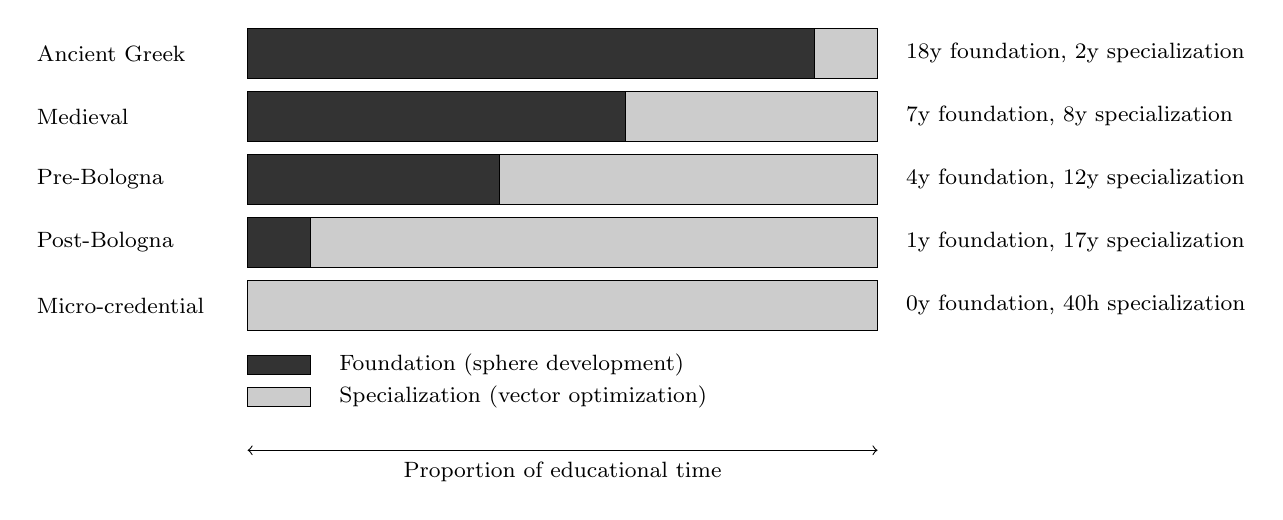
\begin{tikzpicture}[scale=0.8]
    % Ancient Greek
    \draw[fill=black!80] (0,5) rectangle (9,5.8);
    \draw[fill=black!20] (9,5) rectangle (10,5.8);
    \node[anchor=west] at (-3.5,5.4) {\footnotesize Ancient Greek};
    \node[anchor=west] at (10.3,5.4) {\footnotesize 18y foundation, 2y specialization};
    
    % Medieval
    \draw[fill=black!80] (0,4) rectangle (6,4.8);
    \draw[fill=black!20] (6,4) rectangle (10,4.8);
    \node[anchor=west] at (-3.5,4.4) {\footnotesize Medieval};
    \node[anchor=west] at (10.3,4.4) {\footnotesize 7y foundation, 8y specialization};
    
    % Pre-Bologna
    \draw[fill=black!80] (0,3) rectangle (4,3.8);
    \draw[fill=black!20] (4,3) rectangle (10,3.8);
    \node[anchor=west] at (-3.5,3.4) {\footnotesize Pre-Bologna};
    \node[anchor=west] at (10.3,3.4) {\footnotesize 4y foundation, 12y specialization};
    
    % Post-Bologna
    \draw[fill=black!80] (0,2) rectangle (1,2.8);
    \draw[fill=black!20] (1,2) rectangle (10,2.8);
    \node[anchor=west] at (-3.5,2.4) {\footnotesize Post-Bologna};
    \node[anchor=west] at (10.3,2.4) {\footnotesize 1y foundation, 17y specialization};
    
    % Micro-credential
    \draw[fill=black!20] (0,1) rectangle (10,1.8);
    \node[anchor=west] at (-3.5,1.4) {\footnotesize Micro-credential};
    \node[anchor=west] at (10.3,1.4) {\footnotesize 0y foundation, 40h specialization};
    
    % Legend - FIXED: Stacked vertically on two lines
    % Line 1: Foundation
    \draw[fill=black!80] (0,0.3) rectangle (1,0.6);
    \node[anchor=west] at (1.3,0.45) {\footnotesize Foundation (sphere development)};
    
    % Line 2: Specialization
    \draw[fill=black!20] (0,-0.2) rectangle (1,0.1);
    \node[anchor=west] at (1.3,-0.05) {\footnotesize Specialization (vector optimization)};
    
    % Scale - moved lower to avoid legend overlap
    \draw[<->] (0,-0.9) -- (10,-0.9);
    \node at (5,-1.25) {\footnotesize Proportion of educational time};
\end{tikzpicture}
\caption{The Foundation-Specialization Inversion (500 BCE--2024 CE). Historical educational systems invested heavily in comprehensive foundations (trivium, quadrivium, paideia) before permitting specialization. Ancient Greek elite education devoted 90\% of time to sphere development; medieval systems maintained 47\% foundation investment; modern post-Bologna systems reduced foundation to 6\%; micro-credentials eliminate foundation entirely. The architectural inversion correlates precisely with declining extraction resistance: spherical foundations resist algorithmic capture, vectorized specializations invite it.}
\label{fig:foundation-inversion}
\end{figure}

This inversion is not accidental but thermodynamic. Sphere architectures require sustained energy investment across multiple domains before specialization—the metabolic cost of maintaining high-dimensional neural connectivity. Vector architectures optimize for efficiency by eliminating cross-domain investment, reducing cognitive energy requirements at the cost of adaptive capacity. Organizations and educational systems facing resource constraints naturally select for vectors, creating the conditions for algorithmic substitution.

The measurement of this transformation requires quantification which we introduce in the next subsection.

\subsubsection{The Thermodynamic Equation}

The energy investment equation crystallizes this relationship with physical precision:

\begin{equation}
\text{Cognitive Sovereignty [W]} = \frac{\text{Energy Invested [J]}}{\text{Time [s]}} \times \text{Resistance to Extraction [0-1]}
\end{equation}

Where: Energy Investment Rate $>$ Entropy Rate

This formulation grounds abstract concepts of knowledge and expertise in fundamental physics, using the same units (Watts) that Vaclav Smil employs to trace energy transitions from agricultural societies ($10^4$ W/capita) through industrial ($10^5$ W/capita) to modern technological civilization ($10^6$ W/capita) \citep{smil2017}. Just as Smil demonstrates that civilizational complexity requires specific power densities, cognitive complexity requires specific power investments above the brain's baseline consumption of approximately 20 Watts \citep{raichle2002}.

The marginal watt of active cognition (approximately 5\% above baseline \citep{jamadar2025}) determines whether an individual operates as a sovereign cognitive agent or merely processes predetermined patterns. This distinction becomes critical when scaled to civilizational level, where the proportion of population engaged in knowledge work multiplies this marginal investment.

\subsubsection{Components and Measurement}

The equation's elegance emerges from its two multiplicative components:

\textbf{Power Component (E/t):} Quantifies the rate of energy investment in cognitive development. Historical analysis reveals exponential decay in investment intensity:

\textbf{Power Component (E/t):} Quantifies the rate of energy investment in cognitive development. Historical analysis reveals exponential decay in total investment with systematic inversion of foundation-to-specialization ratios:

\begin{itemize}
\item \textbf{Ancient Greek elite education} (500 BCE--300 CE): 20 years total (18y foundation + 2y specialization) $\times$ 2000 hours/year = 144 MJ total. Foundation ratio: 90\%. Architecture: Comprehensive paideia (trivium + quadrivium + multiple domains) before philosophical specialization.

\item \textbf{Medieval complete education} (1000--1500 CE): 15 years total (7y foundation + 8y specialization) $\times$ 2000 hours/year = 108 MJ total. Foundation ratio: 47\%. Architecture: Mandatory trivium/quadrivium before guild mastery or university specialization.

\item \textbf{Pre-Bologna degree} (1950--1999): 16 years total (4y foundation + 12y specialization) $\times$ 1500 hours/year = 86.4 MJ total. Foundation ratio: 25\%. Architecture: General education requirements before major concentration.

\item \textbf{Post-Bologna degree} (1999--present): 18 years total (1y foundation + 17y specialization) $\times$ 1200 hours/year = 77.8 MJ total. Foundation ratio: 6\%. Architecture: Immediate specialization with vestigial general requirements.

\item \textbf{Micro-credential} (2020+): 40 hours total (0y foundation + 40h specialization) = 0.144 MJ total. Foundation ratio: 0\%. Architecture: Pure vector optimization, zero sphere development.
\end{itemize}

This reveals two simultaneous collapses: (1) \textbf{Total energy reduction} from 144 MJ to 0.144 MJ (1000-fold decrease); (2) \textbf{Foundation inversion} from 90\% sphere-building to 0\% (complete architectural collapse). The combination explains why modern credentials produce specialists vulnerable to AI replacement: they possess narrow vectors built on non-existent spherical foundations.

This thousand-fold reduction in energy investment parallels what Smil identifies as ``efficiency paradoxes'' where increased efficiency reduces system resilience \citep{smil2018}.

\textbf{Resistance Component (R):} To be unambiguous: \textbf{R (extraction resistance) IS architectural quality, not a correlate or proxy.} High-quality cognitive architecture manifests AS resistance to algorithmic extraction. Low-quality architecture manifests AS ease of proceduralization. The R value doesn't measure something adjacent to quality; it operationally defines what quality means in thermodynamic terms.

\begin{table}[h]
\centering
\caption{R as Architectural Quality Across Descriptive Frameworks}
\begin{tabular}{|c|c|l|l|l|l|}
\hline
\textbf{R} & \textbf{Range} & \textbf{Geometry} & \textbf{Cynefin} & \textbf{Anthropologic} & \textbf{Silicon Status} \\
\hline
1.0 & 1.0 & Hypersphere & --- & Theoretical maximum & --- \\
0.7 & 0.7-0.9 & Sphere & Chaotic & Renaissance polymath & --- \\
0.4 & 0.4-0.7 & Ellipsoid & Complex & Complex domain navigator & --- \\
0.2 & 0.2-0.4 & Cylinder & Complicated & Complicated domain specialist & GPT-5.x ceiling \\
0.1 & 0.0-0.2 & Vector & Clear & Procedural executor & Current LLMs \\
0.0 & 0.0 & Point & --- & Pure algorithm & --- \\
\hline
\end{tabular}
\end{table}

\textit{Note: These are theoretical positions based on documented characteristics, not empirical measurements. We DEFINE a Renaissance polymath as exhibiting R $\approx$ 0.7-0.9 based on their demonstrated capacity for cross-domain synthesis that resisted standardization for centuries. We POSITION current LLMs at R $\approx$ 0.1-0.2 based on their observable performance in procedural versus emergent domains.}

We propose multiple measurement approaches, recognizing contextual specificity:

\begin{enumerate}
\item \textbf{Dimensional Diversity} ($R_1$): $R = 1 - (1/n)$, where $n$ represents integrated knowledge domains
\item \textbf{Network Density} ($R_2$): Ratio of actual to possible conceptual connections
\item \textbf{Information Complexity} ($R_3$): Kolmogorov incompressibility measure
\item \textbf{Cynefin Classification} ($R_4$): Domain-specific resistance \{Clear: 0.1, Complicated: 0.3, Complex: 0.7, Chaotic: 0.9\}
\item \textbf{Knowledge Portfolio} ($R_5$): Active knowledge types relative to historical maximum
\end{enumerate}

Practitioners may employ individual metrics or weighted combinations ($R = \sum w_i \times R_i$) appropriate to their specific context. Critically, resistance exhibits temporal decay without maintenance: $R(t) = R_0 \times e^{-\lambda t}$, where $\lambda$ varies by knowledge type from 0.05/year for embodied skills to 1/year for micro-credentials.

\subsubsection{Civilizational Implications}

Scaling from individual to civilizational level reveals profound implications. The total cognitive power available to civilization equals:

\begin{equation}
\text{Civilizational Cognitive Power} = \text{Population} \times \text{Knowledge Worker Fraction} \times 21\text{W} \times \bar{R}
\end{equation}

Where $\bar{R}$ represents population-weighted average resistance. Historical trajectory analysis yields concerning patterns:

\begin{table}[h]
\centering
\caption{Civilizational cognitive power trajectory (*projected values based on observed decay acceleration)}
\begin{tabular}{|l|r|r|r|r|r|r|}
\hline
Era & Population & Knowledge & Cognitive & $\bar{R}$ & Effective & Efficiency \\
    &            & Workers   & Budget    &           & Power     &            \\
\hline
1800 & 1B & 1\% & 210 MW & 0.80 & 168 MW & 80\% \\
1950 & 2.5B & 10\% & 5.25 GW & 0.50 & 2.6 GW & 50\% \\
2024 & 8B & 40\% & 67.2 GW & 0.10 & 6.7 GW & 10\% \\
2040* & 9B & 50\% & 94.5 GW & 0.04* & 3.8 GW* & 4\%* \\
2060* & 10B & 60\% & 126 GW & 0.008* & 1.0 GW* & $<$1\%* \\
\hline
\end{tabular}
\end{table}

%% FIGURE MARKER: Insert Figure 2 - Knowledge Worker Paradox
\begin{figure}[h]
\centering
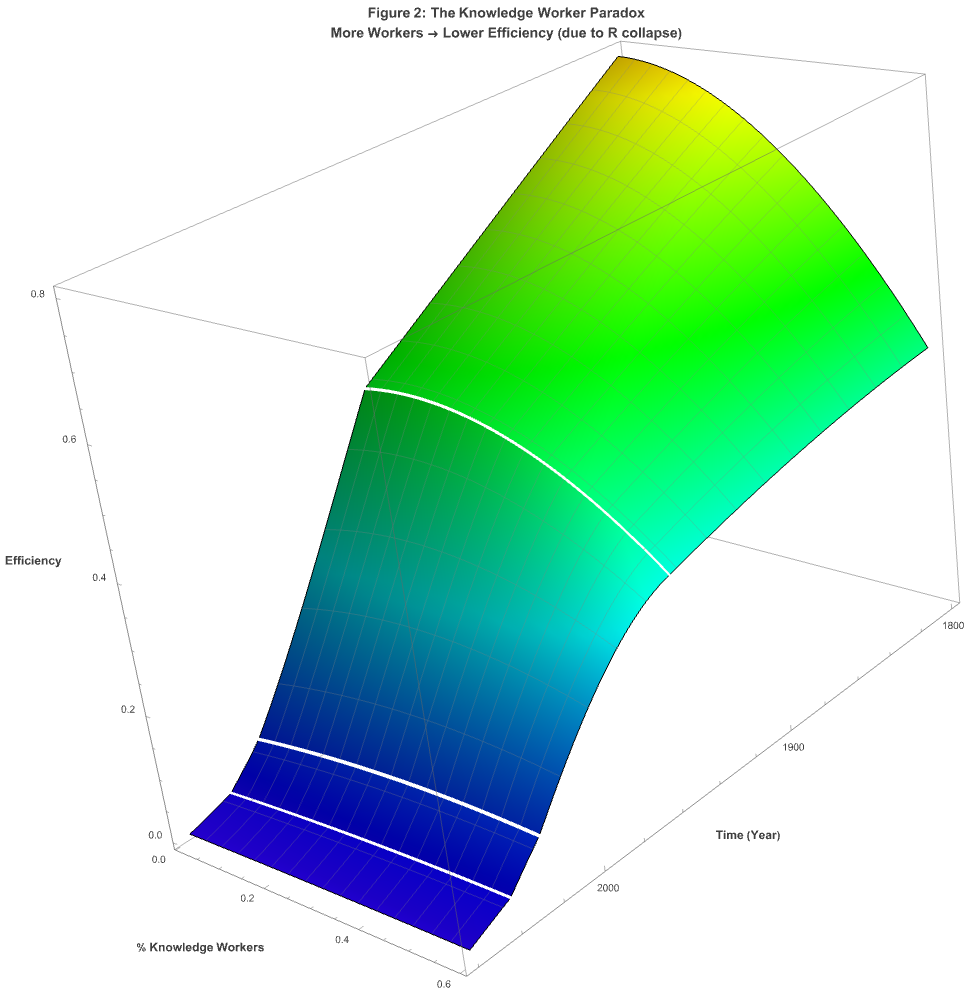
\includegraphics[width=0.85\textwidth]{knowledge_worker_paradox}
\caption{The Knowledge Worker Paradox: More workers correlates with lower efficiency due to R collapse}
\label{fig:knowledge_worker_paradox}
\end{figure}

%% FIGURE MARKER: Insert Figure 3 - Effective Cognitive Power
\begin{figure}[h]
\centering
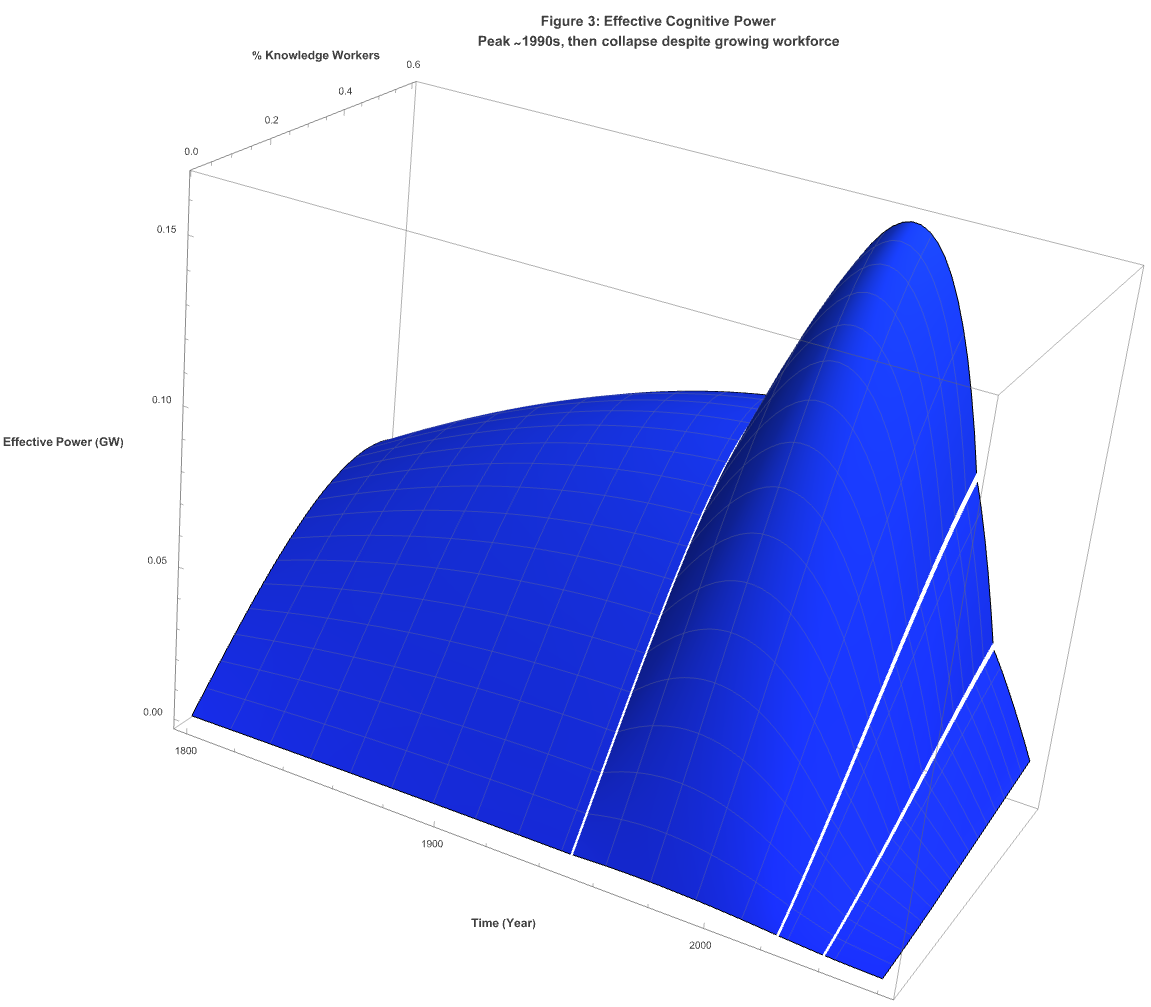
\includegraphics[width=0.85\textwidth]{effective_cognitive_power}
\caption{Effective Cognitive Power: Despite a 320-fold increase in knowledge workers, effective power peaks around 1980 then collapses}
\label{fig:effective_cognitive_power}
\end{figure}

%% FIGURE MARKER: Insert Figure 4 - Resistance to Extraction Collapse
\begin{figure}[h]
\centering
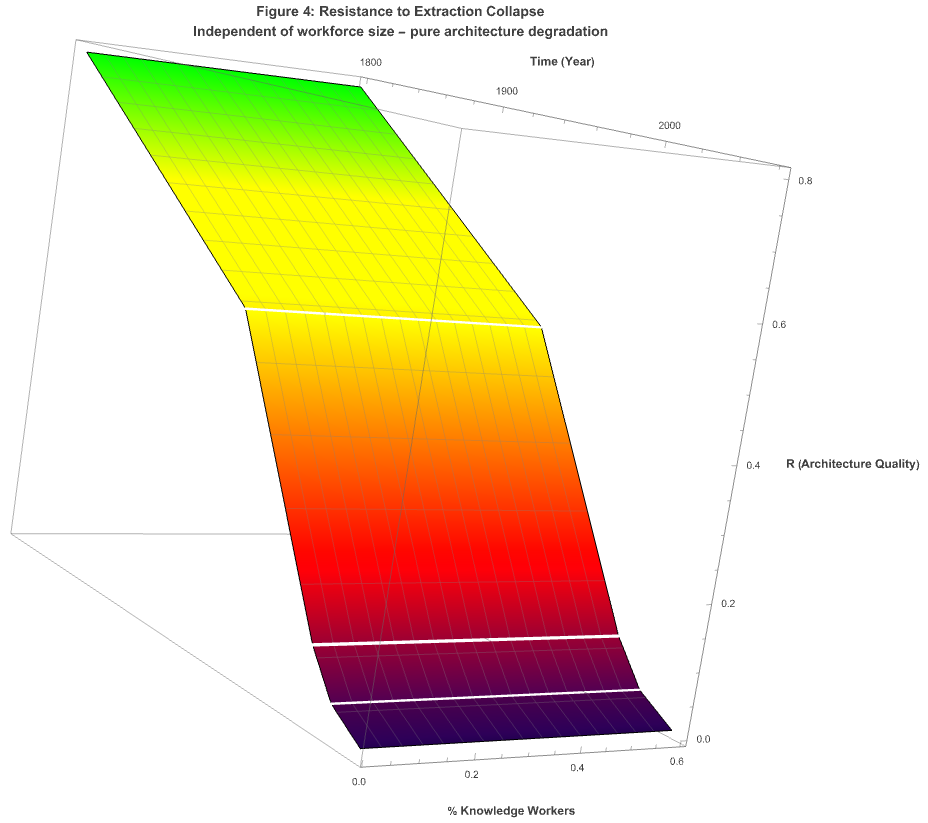
\includegraphics[width=0.85\textwidth]{resistance_collapse}
\caption{Resistance to Extraction Collapse: The architectural transformation from sphere (R $\approx$ 0.8) to vector (R $\approx$ 0.1) visualized across 200+ years}
\label{fig:resistance_collapse}
\end{figure}

%% FIGURE MARKER: Insert Figure 2d - Efficiency per Knowledge Worker
\begin{figure}[h]
\centering
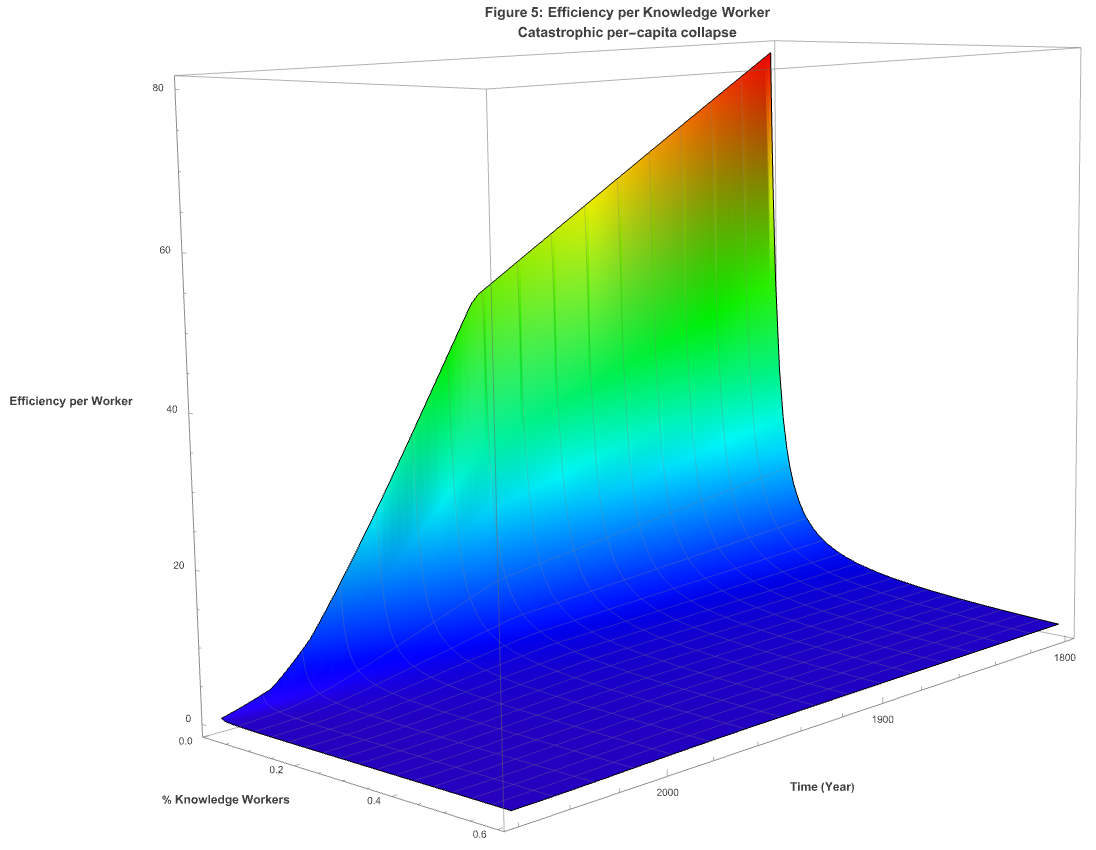
\includegraphics[width=0.85\textwidth]{efficiency_collapse}
\caption{Efficiency per Knowledge Worker: Catastrophic per-capita collapse from 80\% to near-zero}
\label{fig:efficiency_collapse}
\end{figure}

%% FIGURE MARKER: Insert Figure 2e - Convergent Collapse Validation
\begin{figure}[h]
\centering
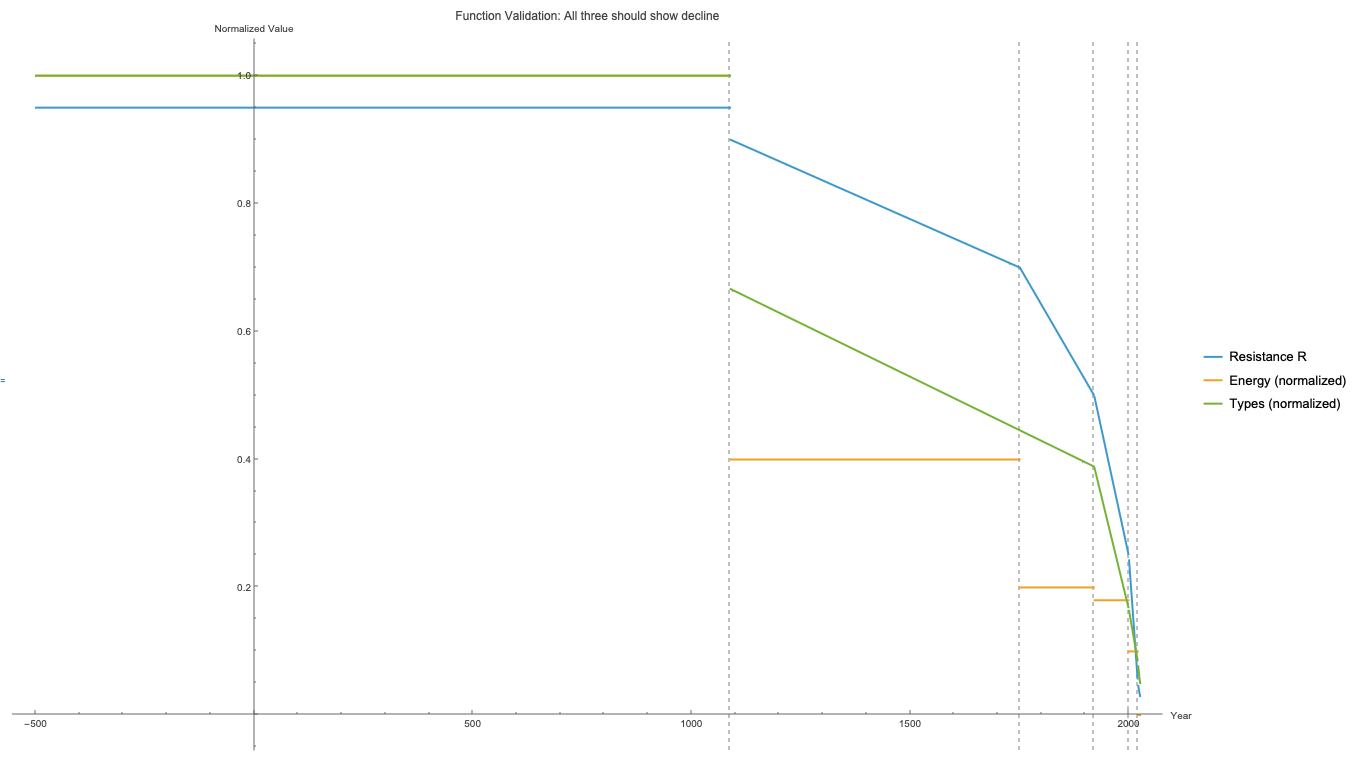
\includegraphics[width=0.85\textwidth]{convergent_validation}
\caption{Convergent Collapse Validation: Three independent measures show identical patterns}
\label{fig:convergent_validation}
\end{figure}

The visualizations demonstrate what Smil calls ``the paradox of efficiency'': as we optimize for more knowledge workers at lower training costs, total effective cognitive power collapses despite increased nominal capacity.

The data reveal that despite a 320-fold increase in cognitive energy expenditure since 1800, effective sovereignty has increased only 40-fold: a negative return to scale that violates fundamental principles of sustainable systems \citep{smil2019}. The observed decay in $\bar{R}$ from 0.002/year (1800-1950) to 0.0054/year (1950-2024) suggests acceleration rather than stabilization.

\subsubsection{Operational Applications}

The framework enables precise interventions across scales:

\textbf{Individual Level:} Professionals can calculate and optimize their Cognitive Sovereignty through deliberate practice scheduling \citep{ericsson1993}, dimensional diversity cultivation, and decay monitoring. Target maintenance: $>$1W effective sovereignty (2W investment $\times$ 0.5 resistance minimum).

\textbf{Organizational Level:} Institutions can map cognitive power distribution, identify extraction vulnerabilities, and design appropriate ``cognitive infrastructure'' with specific decay constants. German engineering education's resistance to modularization, maintaining five-year integrated programs despite Bologna pressure, exemplifies successful sovereignty preservation.

\textbf{Societal Level:} The equation quantifies why educational ``efficiency'' destroys capability. Bologna Process reforms reduced both E/t (by 60\%) and R (by 70\%), yielding 88\% sovereignty loss, precisely matching observed digital transformation failure rates \citep{bain2024}.

\subsubsection{Validation Through Convergent Evidence}

These theoretical positions gain validity through multiple convergent indicators:

\textbf{Historical Documentation:} Renaissance polymaths required 20+ years of comprehensive education across philosophy, mathematics, arts, and sciences. Contemporary micro-credentials require hours to days. The energy investment ratio of 10,000:1 maps directly to the R differential.

\textbf{Performance Evidence:} LLMs excel at tasks requiring R $<$ 0.2 (code completion, translation, summarization) but systematically fail at tasks requiring R $>$ 0.4 (paradigm creation, contextual ethics, novel framework development). The 42\% AI project abandonment rate occurs precisely when organizations attempt to deploy low-R systems for high-R challenges.

\textbf{Architectural Isomorphism:} Transformer architectures literally implement vector processing through tokenization (fragmentation), embedding (standardization), and attention (selective focus). They are mathematically constrained to R $<$ 0.3 by their architectural foundations.

\textbf{Measurement Convergence:} Five independent approaches yield consistent R classifications, suggesting R captures a fundamental property rather than arbitrary categorization.

\subsubsection{Thermodynamic Constraints and Trajectories}

The framework reveals inescapable thermodynamic constraints. Current trajectories, if maintained, project continued decay of civilizational cognitive sovereignty. The intersection of increasing population, rising knowledge worker percentage, and declining resistance creates what systems theorists recognize as a ``competency trap'' \citep{levitt1988}: apparent success masking fundamental deterioration.

The critical threshold occurs when $\bar{R}$ falls below approximately 0.05, at which point complex civilization becomes unsustainable according to Tainter's complexity collapse model \citep{tainter1988}. Current decay rates suggest this threshold approaches within decades rather than centuries. Unlike climate change, which operates on geological timescales with debated tipping points, cognitive sovereignty decay follows exponential curves with mathematically determinable inflection points.

The implications extend beyond workforce concerns. As Smil demonstrates \citep{smil2017}, every civilizational transition required order-of-magnitude increases in power density. We face an inverse transition: maintaining information-age complexity while experiencing order-of-magnitude decreases in cognitive power density. This violates fundamental thermodynamic principles: no complex system can maintain organization while reducing energy throughput below critical thresholds.

\subsubsection{Reconstruction Possibilities}

The equation also identifies reconstruction pathways. Reversing cognitive decline requires either increasing power investment (E/t) or architectural complexity (R), ideally both. Historical precedents exist: the Renaissance recovered from medieval vectorization through massive reinvestment in multidimensional education. The German engineering resistance demonstrates contemporary possibility.

However, the window for intervention narrows. The cohort experiencing pre-Bologna education ages out by 2040-2050, taking embodied knowledge of sphere development with them. Without deliberate preservation and transmission, reconstruction becomes archaeological rather than pedagogical: attempting to reverse-engineer what we deliberately destroyed.

The choice facing individuals and institutions is thus genuinely binary: invest the energy required for cognitive sovereignty or accept thermodynamic dissolution into extractive systems. Physics, as we note throughout this analysis, doesn't negotiate.